\documentclass[11pt, halfparskip]{scrreprt} 

\usepackage{ucs}
\usepackage[utf8x]{inputenc}
\usepackage{ngerman}
\usepackage{amsmath,amssymb,amstext}
\usepackage{graphicx}
\usepackage[automark]{scrpage2}

\title{Project AWT}
\author{Robin Schmid}
\date{14.01.2016}

\begin{document}
\maketitle

\chapter{Initial Position}

\chapter{Technologies}
To create this project, I used several technologies. I will shortly present them in the following sections.
\section{Server}
The application runs on a Glassfish 4.0 Server. The reason I chose Glassfish over Tomcat or others is easy to explain. First I started my Project, but as the structure grew, I had to look out for some more advanced technologies. I then read of CDI (Contexts and Dependency Injection). This is the new standard since Java EE6 and to support Java EE, I had to look out for something else then Tomcat. 

The database is an MySQL database on a simple server provided by XAMPP (locally).

\section{Backend}
For the core of the project I used JSF 2.2. All the necessary dependencies are managed with Maven. Maven is a powerful tool that provides an easy way to find the correct JARS without downloading them manually. One of this dependencies is the JPA (Java Persitence API). I have never work on a Java project with a database behind. So I had to get some information about it. I heard that Hibernate was a good ORM Mapper. I tried it out, but as my project became more and more a EE project, I put down all my effort on Hibernate and chose the reference implementation, EclipseLink. 

\section{Frontend}
For the frontend I completely resigned the use of JSP. I only used Facelets. As I normally work as a frontend developer in my company, I could easily think of some nice extra tools for the frontend. For the most important part, the structure of the pages, I decided to use the Bootstrap framework. To style the pages in my favor, I used the one and only CSS. In stead of writing CSS code directly, I wrote my stylings in SASS. Then with Gulp I builded a minified CSS. With the help of Gulp I could also directly inject dependent style files, for example the already named Bootstrap or Font Awesome for some nice icons. For the dependency management in this part, I used Bower.

\chapter{Project Structure}
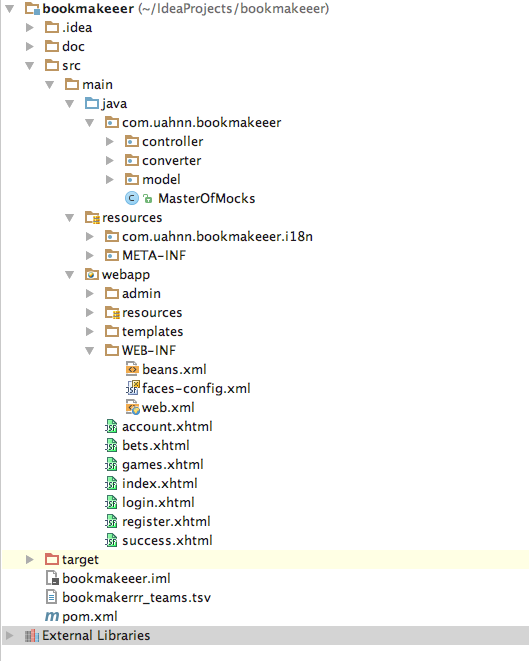
\includegraphics[width=10cm]{project-structure.png}

In the root folder, we have some additional folders, for example the \em{target} folder for the build or the doc folder for versioning the documentation. In source folder (\em{src}) there is the \em{main} directory for the project core. Here would also be possible some tests, but I haven'd had time for that. Then in the \em{main} directory we have the following subfolders:
\begin{itemize}
\item java - for all the java files
\item resources - for i18n files and META-INF
\item webapp - containing the whole frontend part
\end{itemize}

As already written above, the java folder contains all the java files. It contains a package named after my URL. The sub packages are splitted in a minimal order, one for all the backing beans, which I named \em{controller}. All the converter classes are in the \em{converter} package. The whole model, all the JPA entities are in the \em{model} package. I kept it simple and did not write data access object classes (DAO) and accessed the entities directly. This is not very solid and not very clean neither, but it makes accessing the data a bit less complex.

In the \em{src/main/resources} folder we also have a package, named \em{i18n}, containing several resources bundles:
\begin{itemize}
\item bets.properties - Contains the bet type names
\item messages.properties - Contains all messages for errors, etc
\item teams.properties - Contains all team names
\item texts.properties - Contains all other texts, titles, labels
\end{itemize}

I started off with French, German and English, but this is easy to expand. The intelliJ IDE provides a nice interface to edit all texts easily.
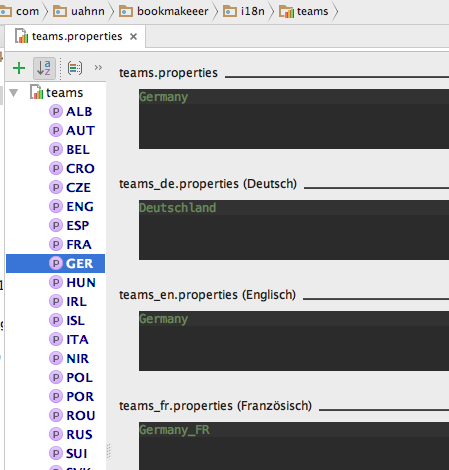
\includegraphics[width=10cm]{i18n-edit.png}

The other resource folder is the \em{META-INF}. It contains the \em{persistence.xml} for the database configuration. 

In the \em{src/main/webapp} we find all frontend files. First of all, the \em{resource} folder holds all the resources like CSS, JS, images or fonts. In my case, I have a \em{dist} subfolder, that contains the builded files. The \em{assets} folder is made for development, here we can write code or put files. Gulp takes those files and builds distribution-ready files (minimized, compressed, etc). 

Another folder is the \em{WEB-INF}, where we have the \em{web.xml}, the \em{beans.xml} and the \em{faces-config.xml}. All those files are for configurate the wep app.

The other folders in the webapp directory are called \em{admin} and \em{templates}. The last holds all templates for the pages. In \em{admin} I put all view for the admin, the manager of the bookmaker. All other views are directly located in the webapp folder. An improvement might be to make an extra folder for all user views. 

\chapter{Components}
Here I will shortly explain all the components of the project. All model classes are located in \em{src/main/java/com.uahnn.bookmakeeer.model}

\section{Model}
\minisec{User}
This entity stores all the information about a user, like e-mail address, firstname, lastname, address, password or balance. It has named queries to return all users, return a user with a given e-mail or all admins.

\minisec{Team}
This entity represents a team competing at the UFEA Euro 2016. It has a ID (FIFA-Shortcode), a UEFA Coefficient and the group, the team was drawn to. We have a named query to return a team by ID or a list of all teams.

\minisec{Game}
Here we have an entity for a Game. A Game as a start time (Date and Time), a home team and an away team. Also we have again named queries to get all upcoming games or all past/started games, that you can no longer bet on.

\minisec{Bet}
The bet entity is the core of the betting system. A bet is always assigned with a game. Every game has multiple bets, one with each bet type. Also every bet has its own odds.

\minisec{UserBet}
This objects maps the bets a user want to make with a given \em{Bet} object and also contains the amount of money a user want to invest for that bet, called the stake.

\section{Controller}
\minisec{RegisterController}
This controller handles the registration of new users. It persists all given Information into the database.

\minisec{LoginController}
This controller manages the login of a user. 

\minisec{GameController}
This controller handles the creation of new games and persists them into the database. It also provides data about the games.

\minisec{BetController}
Within this controller we have the handling of the betting process.

\chapter{Conclusion}
Currently the project is not finished. First of all I have to mention that I had a lot of trouble setting up the database access. This blocked my work, as it was not possible to access any data. I then decided to mock some objects to finally display some data and begin with the frontend development.

I work a lot with web technologies and it found it very disturbing how complicated the whole data access works. I personally think that JSF is a nice way to abstract all components. But it also think that it is meant for business applications. 

\end{document}